\documentclass[12pt]{article}

\usepackage{ishn}

\makeindex[intoc]

\begin{document}

\hypersetup{pageanchor=false}
\begin{titlepage}
	\begin{center}
		\vspace*{1em}
		\Huge
		\textbf{III Quantum Field Theory}

		\vspace{1em}
		\large
		Ishan Nath, Michaelmas 2024

		\vspace{1.5em}

		\Large

		Based on Lectures by Prof. Alejandra Castro

		\vspace{1em}

		\large
		\today
	\end{center}
	
\end{titlepage}
\hypersetup{pageanchor=true}

\tableofcontents

\newpage

% lecture 1

\setcounter{section}{-1}

\section{Introduction}%
\label{sec:intro}

We are following Tong's notes mostly, and Matt Schwartz book for a part of it.

Our goal is to combine quantum mechanics and special relativity. The result is that the number of particles is not preserved.

Key points of this theory is that it is robust and systematic, and governed by a few principles:
\begin{itemize}
	\item locality,
	\item symmetries,
	\item renormalization.
\end{itemize}

There are some units and conventions we will need. In terms of the base units $L, T, M$ (length, time and mass), then
\begin{align*}
	[c] &= [LT^{-1}], \\
	[\hbar] &= [L^2 M T^{-1}], \\
	[G] &= [L^3M^{-1}T^{-2}].
\end{align*}
We take natural units, so $c = 1 = \hbar$, meaning $L = T = M^{-1}$. We refer to the mass dimension of quantities, so $[G] = [M^{-2}] = -2$. Note $M$ also has dimensions of energy.

We will be using the relativistic notation
\[
\eta^{\mu\nu} =
\begin{pmatrix}
	1 & & & \\ & -1 & & \\ & & -1 & \\ & & & -1
\end{pmatrix}.
\]
When talking about spacetime, we let $X^\mu = (t, x, y, z)$.

\newpage

\section{Classical Field Theory}%
\label{sec:classical_ft}

In classical mechanics, a natural object is the action
\[
	S(t_1, t_2) = \int_{t_1}^{t_2} \diff t \, \left( m \sum_{i = 1}^3 \left( \frac{\diff x_i}{\diff t} \right)^2 - V(X^\mu) \right).
\]
Some basic facts of the action is that:
\begin{enumerate}
	\item Equations of motion are given by extremizing $S$.
	\item Boundary conditions are supplied externally.
	\item $S$ is built on symmetries of the system.
\end{enumerate}

We declare in field theory that the fundamental object is a \emph{field}:
\[
	\phi_a(t, \mathbf{x}) : \mathbb{R}^{3, 1} \to \mathbb{R} \text{ or } \mathbb{C} \text{ or } \mathbb{R}^n.
\]
Here $a$ denotes the type of the field. The first consequence is that we are dealing with an infinite number of degrees of freedom.

\begin{exbox}[Electromagnetism]
	In EM, the \emph{gauge field} is
	\[
	A^\mu(x) = (\phi(x), \mathbf{A}(x)).
	\]
	The Maxwell equations are
	\begin{align*}
		\mathbf{E} &= - \nabla \phi - \frac{\partial \mathbf{A}}{\partial t} & \nabla \cdot \mathbf{E} &= \rho, \\
		\mathbf{B} &= \nabla \cdot \mathbf{A}, & \nabla \times \mathbf{B} &= \mathbf{J} + \frac{\partial \mathbf{E}}{\partial t}.
	\end{align*}
	We have two identities:
	\[
	\nabla \cdot \mathbf{B} = 0, \qquad \frac{\diff \mathbf{B}}{\diff t} = \nabla \times \mathbf{E}.
	\]
\end{exbox}

\subsection{Lagrangians}%
\label{sub:lag}

Recall the \emph{Lagrangian} is $L = T - V$, and the action can be written
\[
S = \int \diff t \, L.
\]
We can write
\[
L = \int \Diff3 x \, \mathcal{L}(\phi_a, \partial_\mu \phi_a),
\]
for $\mathcal{L}$ the \emph{Lagrangian density} (or just Lagrangian). Then
\[
S = \int \diff t\, L = \int \Diff4 x \, \mathcal{L}.
\]
The equations of motion can be determined by extremizing over fields. One crucial assumption is that $\mathcal{L}$ depends on $\phi_a$ and $\partial_\mu \phi_a$, and not any higher derivatives. Then,
\begin{align*}
	\delta S &= \int \Diff4 x \left[ \frac{\partial \mathcal{L}}{\partial \phi_a} \delta \phi_a + \frac{\partial \mathcal{L}}{\partial(\partial_\mu \phi_\alpha)} \delta(\partial_\mu \phi_a) \right] \\
		 &= \int \Diff4 x \left[ \frac{\partial \mathcal{L}}{\partial \phi_a} \delta \phi_a - \partial_\mu \left( \frac{\partial \mathcal{L}}{\partial(\partial_\mu \phi_a)} \right) \delta \phi_a + \partial_\mu \left( \frac{\partial \mathcal{L}}{\partial (\partial_\mu \phi_a)} \delta \phi_a \right) \right].
\end{align*}
The last term is a total derivative, and if we assume that fields decay at infinity this evaluates to $0$. Hence requiring $\delta S = 0$ gives
\[
\partial_\mu \left( \frac{\partial \mathcal{L}}{\partial (\partial _\mu \phi_a)} \right) - \frac{\partial \mathcal{L}}{\partial \phi_a} = 0.
\]
\begin{exbox}[Free massive scalar field]
	The `simplest' Lagrangian is
	\begin{align*}
		\mathcal{L} &= \frac{1}{2} \eta^{\mu\nu} \partial_\mu \phi \partial_\nu \phi - \frac{1}{2} m^2 \phi^2 \\
			    &= \frac{1}{2} \dot \phi^2 - \frac{1}{2} ( \nabla \phi)^2 - \frac{1}{2} m^2 \phi^2.
	\end{align*}
	In traditional classical mechanics, the first term is the kinetic energy, and the other two terms give the potential energy.

	In QFT, kinetic terms are any bilinear terms of the fields. So this Lagrangian is all kinetic terms, and no potential terms.

	The equations of motion in this field are
	\[
	\partial_\mu \partial^\mu \phi + m^2 \phi = \square \phi + m^2 \phi = 0.
	\]
	This is the \emph{Klein-Gordon equation}.
\end{exbox}

% lecture 2

\subsection{Hamiltonians}%
\label{sub:ham}

In this setup, one starts by defining the \emph{canonical momentum}\index{canonical momentum}
\[
\Pi^a(x) = \frac{\partial \mathcal{L}}{\partial(\partial_t \phi_a)} = \frac{\partial \mathcal{L}}{\partial \dot \phi_a}.
\]
The \emph{Hamiltonian density}\index{Hamiltonian density} is
\[
\mathcal{H} = \Pi^a \partial_t \phi_a - \mathcal{L}.
\]
The \emph{Hamiltonian}\index{Hamiltonian} is
\[
H = \int \Diff4 x \, \mathcal{H}.
\]

\begin{exbox}[Scalar field with potential]
	Here our Lagrangian is
	\[
	\mathcal{L} = \frac{1}{2} \eta^{\mu \nu} \partial_\mu \phi \partial_\nu \phi - V(\phi).
	\]
	The canonical momentum is
	\[
	\Pi = \frac{\partial \mathcal{L}}{\partial \dot \phi} = \dot \phi.
	\]
	The Hamiltonian is
	\[
	H = \int \Diff4 x \, (\Pi \partial_t \phi - \mathcal{L}) = \int \Diff4 x \left( \frac{1}{2} \dot \phi^2 + \frac{1}{2} (\nabla \phi)^2  + V(\phi) \right).
	\]
\end{exbox}

\subsection{Symmetries}%
\label{sub:sym}

Symmetries will:
\begin{itemize}
	\item Dictate the actions we write.
	\item Dictate the class of fields (operators) used.
	\item Control the observables we will compute.
\end{itemize}

\subsubsection{Lorentz Invariance}%
\label{subsub:lorentz}

The \emph{Lorentz group}\index{Lorentz group} is defined by
\[
x^\mu \to x'^\mu = \Lambda\indices{^{\mu}_{\nu}} x^\nu,
\]
which preserves the interval
\[
s^2 = x^\mu x^\nu \eta_{\mu\nu} = t^2 - \mathbf{x}^2.
\]
So $s^2 \to s'^2 = s^2$. This condition implies that
\[
\eta_{\mu\nu} \Lambda\indices{^{\mu}_{\rho}} \Lambda\indices{^{\nu}_{\sigma}} = \eta_{\rho\sigma},
\]
or in terms of matrices,
\[
\Lambda^T \eta \Lambda = \eta.
\]

\begin{exbox}
	\begin{enumerate}
		\item Rotations: Say $t' = t$, and $\Lambda\indices{^{i}_{j}} = R\indices{^{i}_{j}}$, for $R \in O(3)$. A rotation in the $x$-$y$ plane is given by
		\[
		\Lambda =
		\begin{pmatrix}
			1 & 0 & 0 & 0 \\
			0 & \cos \theta & - \sin \theta & 0 \\
			0 & \sin \theta & \cos \theta & 0 \\
			0 & 0 & 0 & 1
		\end{pmatrix}.
		\]
	\item Boosts: these mix time and space. A boost in the $(t, x)$ plane is
		\[
		\Lambda =
		\begin{pmatrix}
			\cosh \eta & - \sinh \eta & 0 & 0 \\
			- \sinh \eta & \cosh \eta & 0 & 0 \\
			0 & 0 & 1 & 0 \\
			0 & 0 & 0 & 1
		\end{pmatrix}.
		\]
		Here $\eta$ is the rapidity, and
		\[
			\cosh \eta = \frac{1}{\sqrt{1 - v^2}}, \qquad \sinh \eta = \frac{v}{\sqrt{1 - v^2}}.
		\]
	\end{enumerate}
\end{exbox}

More generally, if we take the determinant of $\Lambda^T \eta \Lambda = \eta$, we find
\[
\det (\Lambda)^2 = 1 \implies \det \Lambda = \pm 1.
\]
If $\det \Lambda = 1$, this is called a \emph{proper Lorentz transformation}\index{Lorentz transformation}. If $\det \Lambda = -1$, this is a \emph{improper Lorentz transformation}.

Proper Lorentz transformations can be continuously connected to the identity, whereas improper Lorentz transformation include symmetries such as parity, and time reversal.

If we focus on $\det \Lambda = 1$, we can then write
\[
\Lambda\indices{^{\mu}_{\nu}} = \delta\indices{^{\mu}_{\nu}} + \eps\indices{^{\mu}_{\nu}} + \mathcal{O}(\eps^2).
\]
What are the properties of $\eps\indices{^{\mu}_{\nu}}$? Plugging this formula into the definition of a Lorentz transformation, we find
\begin{align*}
	\eta_{\rho\sigma} &= \eta_{\mu\nu} (\delta\indices{^{\mu}_{\rho}} + \eps\indices{^{\mu}_{\rho}} + \cdots)(\delta\indices{^{\nu}_{\sigma}} + \eps\indices{^{\nu}_{\sigma}} + \cdots) \\
			  &= \eta_{\mu\nu} \delta\indices{^{\mu}_{\rho}} \delta\indices{^{\nu}_{\sigma}} + \eta_{\mu\nu} \eps\indices{^{\mu}_{\rho}} \delta\indices{^{\nu}_{\sigma}} + \eta_{\mu\nu} \delta\indices{^{\mu}_{\rho}} \eps\indices{^{\nu}_{\sigma}} + \mathcal{O}(\eps^2) \\
			  &= \eta_{\rho\sigma} + \eps_{\sigma\rho} + \eps_{\rho\sigma} + \cdots
\end{align*}
Hence $\eps_{\sigma\rho} = - \eps_{\rho\sigma}$, which gives an anti-symmetric tensor. Therefore, in 3+1 dimensions, we have 6 components. Therefore, we have 6 generators for the Lorentz group, 3 rotations and 3 boosts.

In this context, a field is an object that depends on some coordinates, and has a definite transformation under Lorentz: if $x \to x' = \Lambda x$, then
\[
	\phi_a(x) \to \phi_a'(x) = D[\Lambda]\indices{_{a}^b} \phi_b(\Lambda^{-1}x).
\]
Here $D$ forms a representation of the Lorentz group, so
\begin{itemize}
	\item $D[\Lambda_1] D[\Lambda_2] = D[\Lambda_1 \Lambda_2]$,
	\item $D[\Lambda^{-1}] = D[\Lambda]^{-1}$,
	\item $D[1] = 1$.
\end{itemize}

In the above, we have $\phi_b(\Lambda^{-1}x)$. Why are we using the active transformation? Consider a trivial representation $D[\Lambda] = 1$. Then we want
\[
\phi'(x) = \phi(\Lambda^{-1} x).
\]
This is the definition of the scalar field.

\begin{center}
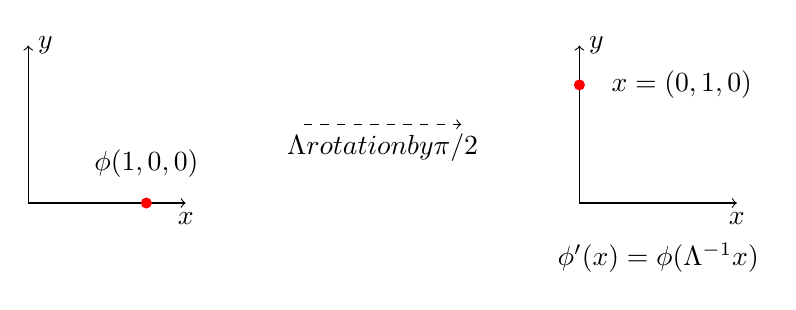
\begin{tikzpicture}
    % R^n axes
    \draw[->] (-4.5,0) -- (-2.5,0) node[anchor=north] {$x$};
    \draw[->] (-4.5,0) -- (-4.5,2) node[anchor=west] {$y$};
    \fill[red] (-3,0) circle (2pt);
    \node at (-3, 0.5) {$\phi(1, 0, 0)$};

    % R^{n'} axes
    \draw[->] (2.5,0) -- (4.5,0) node[anchor=north] {$x$};
    \draw[->] (2.5,0) -- (2.5,2) node[anchor=west] {$y$};
    \fill[red] (2.5,1.5) circle (2pt);
    \node at (3.5, -0.7) {$\phi'(x) = \phi(\Lambda^{-1}x)$};
    \node at (3.8, 1.5) {$x = (0, 1, 0)$};

    % Dashed arrow for the map between R^n and R^{n'}
    \draw[->, dashed] (-1,1) -- (1,1) node[midway,below] {$\Lambda \text{ rotation by } \pi/2$};


\end{tikzpicture}
\end{center}

\begin{exbox}
	The trivial representation gives a scalar field.

	Another example is a vector representation, so
	\[
		D[\Lambda] \indices{^{\mu}_{\nu}} = \Lambda\indices{^{\mu}_{\nu}}.
	\]
	So then
	\[
	A^\mu(x) \to A'^\mu(x) = \Lambda\indices{^{\mu}_{\nu}} A^\nu(\Lambda^{-1}x),
	\]
	and
	\[
	\partial_\mu \phi \to \partial_\mu \phi'(x) = (\Lambda^{-1})\indices{^{\mu}_{\nu}} \partial_\mu \phi(\Lambda^{-1}x).
	\]
\end{exbox}

Now we will see how symmetries constrain actions. For example consider
\[
\mathcal{L} = \frac{1}{2} \partial_\mu \phi \partial_\nu \phi \eta^{\mu\nu} - \frac{1}{2} m^2 \phi^2, \qquad S = \int \Diff 4 x \, \mathcal{L}.
\]
We can verify this is invariant under Lorentz.

% lecture 3

Note under the Lorentz transformation, the fields transform as
\begin{align*}
	\phi(x) &\to \phi(x) = \phi(\Lambda^{-1}x) = \phi(y), \\
	\partial_\mu \phi &\to (\Lambda^{-1})\indices{^{\nu}_{\mu}} \partial_\nu \phi(y).
\end{align*}
If we replace this in the Lagrangian,
\begin{align*}
	\mathcal{L} &\to \frac{1}{2}(\Lambda^{-1})\indices{^{\rho}_{\mu}} \partial_\mu \phi(y) (\Lambda^{-1})\indices{^{\sigma}_{\nu}} \partial_\sigma \phi(y) - \frac{1}{2} m^2 \phi^2(y) \\
		    &= \frac{1}{2} \eta^{\rho\sigma} \partial_\rho \phi \partial_\sigma \phi - \frac{1}{2} m^2 \phi^2.
\end{align*}
Therefore,
\[
\mathcal{L}(x) \to \mathcal{L}'(x) = \mathcal{L}(y).
\]
Hence
\[
S = \int \Diff4 x \, \mathcal{L}(x) \to \int \Diff4 x \, \mathcal{L}(y) = \int \Diff4 y\, \mathcal{L}(y)
\]
is conserved (note the change in variable $x \to y$ has Jacobian 1, as $\det \Lambda = 1$).

\subsection{N\"oether's Theorem}%
\label{sub:nt}

This has two parts:
\begin{enumerate}
	\item Every continuous symmetry of the Lagrangian gives rise to a current $j^\mu$, and the equations of motions imply
		\[
		\partial_\mu j^\mu = 0 \implies \frac{\partial j^0}{\partial t} + \nabla \cdot j^i = 0.
		\]
	\item Provided suitable boundary conditions,  a conserved current will give rise to a conserved charge $Q$, where
		\[
		Q = \int \Diff 3x \,j^0.
		\]
\end{enumerate}

\begin{definition}
	A transformation is \emph{continuous} if there is an infinitesimal parameter in it. They can either be:
	\begin{itemize}
		\item internal: they do not act on the coordinates, but instead on the fields.
		\item local: they act on the coordinates and the fields.
	\end{itemize}
	In both cases, the differential of a continuous transformation is
	\[
	\delta \phi_a = \phi_a'(x) - \phi_a(x).
	\]
	Such a transformation is a symmetry of the system if the action is invariant, so
	\[
	S[\phi] \to S[\phi'] = \int \Diff4 x\, \mathcal{L}(x),
	\]
	and moreover
	\[
		\delta(S) = S[\phi'] - S[\phi] = 0.
	\]
	This implies that for the Lagrangian,
	\[
	\delta \mathcal{L} = \mathcal{L}'(x) - \mathcal{L}(x) = \partial_\mu F^\mu,
	\]
	the same up to a total derivative.
\end{definition}

\begin{proofbox}
	Let us quantify the change in $\mathcal{L}$:
	\begin{align*}
		\delta \mathcal{L} &= \frac{\partial \mathcal{L}}{\partial \phi_a}  \delta \phi_a + \frac{\partial \mathcal{L}}{\partial \partial_\mu \phi_a} \delta \partial_\mu \phi_\alpha \\
				   &= \left( \frac{\partial \mathcal{L}}{\partial \phi_a} - \partial_\mu \left( \frac{\partial \mathcal{L}}{\partial \partial_\mu \phi_a} \right) \right) \delta \phi_a + \partial_\mu \left( \frac{\partial \mathcal{L}}{\partial \partial_\mu \phi_a} \delta \phi_\alpha \right) = \partial_\mu F^\mu,
	\end{align*}
	as it is a symmetry. Hence,
	\[
		- \left( \frac{\partial \mathcal{L}}{\partial \phi_a} - \partial_\mu \left( \frac{\partial \mathcal{L}}{\partial \partial_\mu \phi_a} \right) \right) \delta \phi_a = \partial_\mu \underbrace{\left( \frac{\partial \mathcal{L}}{\partial \partial_\mu \phi_a} \delta \phi_a - F^\mu \right)}_{j^\mu}.
	\]
	If the equations of motion are imposed, then
	\[
	\partial_\mu j^\mu = 0,
	\]
	where
	\[
	j^\mu = \frac{\partial \mathcal{L}}{\partial \partial_\mu \phi_\alpha} \delta \phi_a - F^\mu.
	\]
	For the second part of the statement, we have
	\[
	Q = \int \Diff 3 x \, j_0.
	\]
	Then the total time derivative is
	\[
	\frac{\diff Q}{\diff t} = \int_V \Diff3 x\, \frac{\partial j^0}{\partial t} = - \int_V \Diff3 x \, \nabla \cdot j = - \int_{\partial V} \diff A \cdot j = 0,
	\]
	given suitable boundary conditions on $j$, i.e. fields decay.
\end{proofbox}

\subsection{Energy-Momentum Tensor}%
\label{sub:em_t}

Consider local transformations given by translations:
\[
x^\mu \to x'^\mu = x^\mu - \eps^\mu.
\]
Under translation, the fields transform as
\[
\phi_a(x) \to \phi_a'(x) = \phi_a(x + \eps) = \phi_a(x) + \eps^\mu \partial_\mu \phi_a + \mathcal{O}(\eps^2).
\]
Hence we find
\[
\delta \phi_a = \phi_a'(x) - \phi_a(x) = \eps^\mu \partial_\mu \phi_a.
\]
The Lagrangian changes as
\[
\delta \mathcal{L} = \eps^\mu \partial_\mu \mathcal{L} = \partial_\mu (\eps^\mu \mathcal{L}).
\]
The conserved current is then
\begin{align*}
	j^\mu &= \frac{\partial \mathcal{L}}{\partial(\partial_\mu \phi_a)} \eps^\nu \partial_\nu \phi_a - \eps^\mu \mathcal{L} \\
	      &= \eps^\nu \left( \frac{\partial \mathcal{L}}{\partial (\partial_\mu \phi_a)} \partial_\nu \phi_a - \delta\indices{^{\mu}_{\nu}} \mathcal{L} \right) \\
	      &= \eps^\nu T\indices{^{\mu}_{\nu}},
\end{align*}
where $T\indices{^{\mu}_{\nu}}$ is the energy-momentum tensor. If the equations of motion are 0, then varying $\eps^\nu$, we find
\[
\partial_\mu j^\mu = 0 \implies \partial_\mu T\indices{^{\mu}_{\nu}} = 0.
\]
We can construct four conserved charges:
\begin{align*}
	E &= \int \Diff3 x \, T^{00}, \\
	P^i &= \int \Diff 3 x \, T^{0i}.
\end{align*}
These are the energy, and the three momenta.

\begin{exbox}[Free massive scalar field]
	Here we have
	\[
	T\indices{^{\mu}_{\nu}} = \frac{\partial \mathcal{L}}{\partial (\partial_\mu \phi_a)} \partial_\nu \phi - \delta\indices{^{\mu}_{\nu}} \mathcal{L},
	\]
	so
	\[
	T^{\mu\nu}= \partial^\mu \phi \partial^\nu \phi - \eta^{\mu\nu} \mathcal{L}.
	\]
	Then we find
	\[
	T^{00} = \frac{1}{2} \dot \phi^2 + \frac{1}{2} (\nabla \phi)^2 + \frac{1}{2} m^2 \phi^2.
	\]
	So
	\[
	E = \int \Diff 3 x \, T^{00} = H, \qquad p^i = \int \Diff 3 x \, T^{0i} = \int \Diff 3x \, \dot \phi \partial^i \phi.
	\]
\end{exbox}

\begin{remark}
	The definition of the EM tensor is
	\[
	T\indices{^{\mu}_{\nu}} = \frac{\partial \mathcal{L}}{\partial (\partial_\mu \phi_a)} \partial_\nu \phi_a - \delta\indices{^{\mu}_{\nu}} \mathcal{L}.
	\]
	From this equation, we do not ensure that $T$ is symmetric. How can we make it symmetric?
	\begin{enumerate}
		\item Define
			\[
			\Theta^{\mu\nu} = T^{\mu\nu} + \partial_\rho \Gamma^{\rho\mu\nu},
			\]
			where
			\[
			\Gamma^{\rho\mu\nu}= - \Gamma^{\mu\rho\nu},
			\]
			such that $\partial_\mu \Theta^{\mu\nu} = 0$.
		\item Couple fields to $g_{\mu\nu}$. Then
			\[
			\Theta^{\mu\nu} = \left( - \frac{2}{\sqrt{-g}} \frac{\partial}{\partial g_{\mu\nu}} \left( \sqrt{-g} \mathcal{L} \right) \right) \biggr|_{g = \eta}.
			\]
	\end{enumerate}
	
\end{remark}

% lecture 4

\begin{exbox}[Complex scalar field]
	A complex scalar field is
	\[
	\psi(x) = \frac{1}{\sqrt 2} (\phi_1(x) + i \phi_2(x)),
	\]
	where $\phi_i$ are real scalar fields. A Lagrangian for this field is
	\[
	\mathcal{L} = \frac{1}{2} \partial_\mu \psi \partial^\mu \psi^\ast - V(|\psi|^2).
	\]
	The equations of motion turn out to be
	\[
	\partial_\mu \partial^\mu \psi + \frac{\partial V}{\partial \psi^\ast} = 0, \qquad \partial_\mu \partial^\mu \psi^\ast + \frac{\partial V}{\partial \psi} = 0.
	\]
	In this system, there is an internal symmetry given by
	\[
	\psi(x) \to \psi'(x) = e^{i \alpha} \psi(x), \qquad \psi^\ast (x) \to \psi'^\ast (x) = e^{-i\alpha} \psi^\ast(x).
	\]
	Here $\mathcal{L} \to \mathcal{L}' = \mathcal{L}$, so $\mathcal{S} \to \mathcal{S}' = \mathcal{S}$.

	$\alpha$ is a continuous parameter of the transformation, so $\delta \psi = \psi'(\alpha) - \psi(\alpha) = i \alpha \psi$, and $\delta \psi^\ast = -i\alpha \psi^\ast$.

	We can construct the current as
	\begin{align*}
		j^\mu &= \frac{\partial \mathcal{L}}{\partial \partial_\mu \psi} \delta \psi + \frac{\partial \mathcal{L}}{\partial \partial_\mu \psi^\ast} \delta \psi^\ast \\
		      &= \partial^\mu \psi^\ast \delta \psi + \partial^\mu \psi \delta \psi^\ast \\
		      &= i \alpha(\psi \partial^\mu \psi^\ast - \psi^\ast \partial^\mu \psi).
	\end{align*}
	It is also possible to parametrize our transformation as
	\[
	\begin{pmatrix}
		\phi_1 \\ \phi_2
	\end{pmatrix}
	\to
	\begin{pmatrix}
		\phi_1' \\ \phi_2'
	\end{pmatrix} =
	\begin{pmatrix}
		\cos \alpha & -\sin\alpha \\ \sin \alpha & \cos \alpha
	\end{pmatrix}
	\begin{pmatrix}
		\phi_1 \\ \phi_2
	\end{pmatrix}.
	\]
\end{exbox}

\newpage

\section{Quantum Fields}%
\label{sec:qf}

\subsection{Free Theory}%
\label{sub:qfft}

We will begin by taking a Hamiltonian approach, and will follow the rules of QM. In this framework,
\[
	[X^i, P^j] = i \hbar \delta^{ij}.
\]
In QFT, we now have $\phi_a(x)$ and $\Pi^a(x)$, where $\Pi^a = \partial \mathcal{L} / \partial \phi_a$. The new rule is
\[
	[\phi_a(\mathbf{x}, t), \Pi^b(\mathbf{x}, t)] = i \delta^3(\mathbf{x} - \mathbf{y}) \delta\indices{^{b}_{a}}.
\]
This looks like it breaks relativity; we will see it does not. Our goal is to implement such a quantum field theory for the free massive real scalar field. The plan will be to go through:
\begin{itemize}
	\item Canonical quantization.
	\item Hamiltonian.
	\item Fock space.
	\item Causality.
	\item Propagators.
\end{itemize}

\subsection{Canonical Quantization}%
\label{sub:cq}

Our theory is
\[
\mathcal{L} = \frac{1}{2} \partial_\mu \phi \partial^\mu \phi - \frac{1}{2} m^2 \phi^2.
\]
The equations of motion are
\[
\partial_\mu \partial^\mu \phi + m^2 \phi = 0.
\]
Solutions to this include
\[
\phi \sim \exp\left( i \mathbf{k} \cdot \mathbf{x} + i \omega t\right),
\]
where $\omega, \mathbf{k}, m$ are related by
\[
	-\omega^2 + \mathbf{k}^2 + m^2 = 0 \implies \omega = \pm \sqrt{\mathbf{k}^2 + m^2}.
\]
We adopt the notation
\[
	\omega = \sqrt{\mathbf{k}^2 + m^2}.
\]
Hence, we can write
\[
	\phi(\mathbf{x}, t) = \int \frac{\Diff3 k}{(2 \pi)^3} \left[ a(\mathbf{k}) e^{i \mathbf{k} \cdot \mathbf{x} - i \omega t} + b(\mathbf{k}) e^{i \mathbf{k} \cdot \mathbf{x} + i \omega t} \right].
\]
Note that $\phi$ is real, so $\phi^\ast = \phi$ implies
\[
a^\ast(- \mathbf{k}) = b(\mathbf{k}), \qquad b^\ast(-\mathbf{k}) = a(\mathbf{k}).
\]
Hence we can write
\begin{align*}
	\phi(x) &= \int \frac{\Diff3 k}{(2 \pi)^3} \left[ a(\mathbf{k}) e^{i \mathbf{k} \cdot \mathbf{x} - i \omega t} + a^\ast(\mathbf{k}) e^{-i \mathbf{k} \cdot \mathbf{x} + i \omega t} \right] \\
		&= \int \frac{\Diff3 k}{( 2\pi)^3} \left[ a(\mathbf{k}) e^{-ikx} + a^\ast(\mathbf{k}) e^{ik x} \right],
\end{align*}
where
\[
kx = k^\mu x_\mu = \omega t - \mathbf{k} \cdot \mathbf{x}, \qquad k^2 = \omega^2 - \mathbf{k}^2 = m^2.
\]
We choose to normalize $a(\mathbf{k})$ and $a^\ast(\mathbf{k})$ such that
\[
	\phi(x) = \int \frac{\Diff 3k}{(2\pi)^3} \frac{1}{\sqrt{2 \omega}} \left[ a(\mathbf{k}) e^{-ikx} + a^\ast(\mathbf{k}) e^{ikx}\right].
\]
Next, we quantize. To do this, we calculate the conjugate momenta:
\[
	\Pi(x) = \dot \phi = \int \frac{\Diff3k}{(2\pi)^3} \frac{1}{i}\sqrt{\frac \omega2} \left[ a(\mathbf{k}) e^{-ikx} - a^\ast(\mathbf{k})e^{ikx}\right].
\]
We declare
\begin{align*}
	[\phi(\mathbf{x}, t), \phi(\mathbf{x}', t)] &= 0,\\
	[\Pi(\mathbf{x},t), \Pi(\mathbf{x}',t)] &= 0,\\
	[\phi(\mathbf{x}, t), \Pi(\mathbf{x}', t)] &= i \delta^3(\mathbf{x} - \mathbf{x}').
\end{align*}
The claim is that these commutation relations promote $a$ to an operator, and $a^\ast$ becomes $a^\dagger$, also an operator. These themselves have commutation relations:
\begin{align*}
	[a(\mathbf{k}), a(\mathbf{k}')] &= 0,\\
	[a^\dagger(\mathbf{k}), a^\dagger(\mathbf{k}')] &= 0,\\
	[a(\mathbf{k}), a^\dagger(\mathbf{k}')] &= (2 \pi)^3 \delta^3(\mathbf{k} - \mathbf{k}').
\end{align*}

\begin{proofbox}
	We show that the second set of commutation relations imply the first set. We only prove the last one as it is the only non-trivial one:
	\begin{align*}
		[\phi(\mathbf{x}, t), \Pi(\mathbf{y}, t)] &= \int \frac{\Diff3 p \Diff 3 q}{(2 \pi)^6} \frac{1}{2i} \sqrt{\frac{\omega_p}{\omega_q}} \bigl( \bigl[ a(p) e^{i \mathbf{p} \cdot \mathbf{x} - i \omega t} + a^\dagger (p) e^{-i \mathbf{p} \cdot \mathbf{x} + i \omega t}, \\
							  &\qquad \qquad \qquad a(q) e^{i \mathbf{q} \cdot \mathbf{y} - i \omega t} - a^\dagger(q) e^{-i \mathbf{q} \cdot \mathbf{y} + i \omega t} \bigr] \bigr) \\
							  &= C \int \Diff3 p \Diff3 q \bigl( - [a(p), a^\dagger(q)] e^{i \mathbf{p} \cdot \mathbf{x}} e^{-i \mathbf{q} \cdot \mathbf{y}} e^{it(\omega_q - \omega_p)} \\
							  & \qquad \qquad \qquad \qquad + [a^\dagger(p), a(q)] e^{-i \mathbf{p} \cdot \mathbf{x}} e^{i \mathbf{q} \cdot \mathbf{y}} e^{it(\omega_p - \omega_q)} \bigr) \\
							  &= i \int \frac{\Diff 3 p}{(2 \pi)^3} e^{i p (\mathbf{x} - \mathbf{y})} = i \delta^3(\mathbf{x} - \mathbf{y}).
	\end{align*}
\end{proofbox}

% lecture 5

\subsection{Hamiltonian}%
\label{sub:hqft}

The Hamiltonian of the free theory is
\[
	H = \int \Diff3 x \, \mathcal{H} = \frac{1}{2} \int \Diff 3 x\,(\Pi^2 + (\nabla \phi)^2 + m^2 \phi^2),
\]
which we want in terms of $a, a^\dagger$. Writing this out,
\begin{align*}
	H &= \frac{1}{2} \int \Diff 3 x \int \frac{\Diff 3 p \Diff 3 q}{(2\pi)^6} \biggl( - \frac{\sqrt{\omega_p \omega_q}}{2} (a e^{-ipx} - a^{\dagger} e^{ipx})(ae^{-iqx} - a^{\dagger} e^{iqx}) \\
	  & \qquad \qquad - \frac{1}{2} \frac{1}{\sqrt{\omega_p \omega_q}} (a e^{-ipx} - a^{\dagger} e^{ipx})(a e^{-iqx} - a^\dagger e^{iqx}) \mathbf{p} \cdot \mathbf{q} \\
	  & \qquad \qquad + \frac{m^2}{2} \frac{1}{\sqrt{\omega_p \omega_q}} (a e^{ipx} + a^{\dagger} e^{-ipx})(ae^{iqx} + a^{\dagger} e^{-iqx}) \biggr) \\
	  &= \frac{1}{2} \int \frac{\Diff 3 p}{(2 \pi)^3} \frac{1}{2 \omega_p} \biggl[ \underbrace{(-\omega_p^2 + \mathbf{p}^2 + m^2)}_{0}(a_p a_p e^{-2i\omega t} + a_p^{\dagger} a_p^{\dagger} e^{2i\omega t}) \\
	  & \qquad \qquad + (\omega_p^2 + \mathbf{p}^2 + m^2)(a_p^\dagger a_p + a_p a_p^\dagger) \biggr] \\
	  &= \frac{1}{2} \int \frac{\Diff 3p}{(2 \pi)^3} \omega(a_p^\dagger a_p + a_p a_p^\dagger) \\
	  &= \int \frac{\Diff 3 p}{(2 \pi)^3} \omega a_p^\dagger a_p + \int \frac{\Diff 3 p}{2} \, \omega \delta(0).
\end{align*}
We should be scared by the last term. If we take a vacuum state $\ket 0$ such that
\[
a_p \ket 0 = 0,
\]
then in fact
\[
H \ket 0 = \int \frac{\Diff 3 p}{2} \omega (2 \pi)^3 \delta(0) \ket 0 = \infty.
\]
To understand the nature of this, we need to see the origin of this divergence. We actually have two infinities:
\begin{enumerate}[(i)]
	\item Infrared divergence: $(2 \pi)^3 \delta(0)$. This arises as follows:
		\[
			(2\pi)^3 \delta(0) = \lim_{L \to \infty} \int_{-L}^L \Diff 3 x e^{i \mathbf{x} \cdot \mathbf{p}} \biggr|_{\mathbf{p} = 0} = \lim_{L \to \infty} \int_{-L}^{L} \Diff 3 x = V.
		\]
		For an infinite size system, this blows up. The solution is to discuss energy densities, so
		\[
		\mathcal{E}_0 = \frac{E_0}{V} = \int \frac{\Diff 3p}{(2 \pi)^3} \, \frac{1}{2} \omega_p \sim \int \Diff 3 p \, p^{2} \to \infty.
		\]
		This also diverges.
	\item Ultraviolet divergence:
		\[
			\int_0^{p_{\mathrm{max}}} \Diff 3 p \, \sqrt{p^2 + m^2} \to \infty,
		\]
		which is high-frequency divergence.

		It is absurd to think that the theory is valid for arbitrarily high energies.
\end{enumerate}

The solution, which is mostly practical, is to declare
\[
H = \int \frac{\Diff 3 p}{(2 \pi)^3} \, \omega_p a_p^\dagger a_p,
\]
and with this $H \ket 0 = 0$.

The origin is due to an ambiguity in multiplying fields. The cure is \emph{normal ordering}\index{normal ordering}.

\begin{definition}
	If we are given a list of fields, we define the \emph{normal ordering} as
	\[
	: \phi_1(x_1) \phi_2(x_2) \cdots \phi_n(x_n):
	\]
	where this is the usual product with all $a(p)$ operators placed to the right of an $a^\dagger(p)$.
\end{definition}

\subsection{Fock Space}%
\label{sub:fs}

Given $\ket 0$, we want to construct excited states. We know
\begin{align*}
	[H, a_p^\dagger] &= \omega_p a_p^\dagger, \\
	[H, a_p] &= \omega_p a_p.
\end{align*}
We can construct excited states by
\begin{align*}
	\ket p &= a^\dagger(p) \ket 0, \\
	H \ket p &= \omega_p \ket p,
\end{align*}
% lecture 6
where $\omega_p^2 = p^2 + m^2$. We can consider
\[
\mathbf{P} = - \int \Diff3 x \pi \nabla \phi = \int \frac{\Diff 3 k}{(2 \pi)^3} k a_k^\dagger a_k,
\]
where
\[
	\mathbf{P}\ket{\mathbf{p}}= \mathbf{p} \ket{\mathbf{p}}.
\]
Here $\ket{\mathbf{p}}$ is a momentum and energy eigenstate, with eigenvalues $\mathbf{p}$ and energy $E = w_p^2 = \mathbf{p}^2 + m^2$.

Also, $\mathbf{p} = 0$ is an angular momentum $J^i$ eigenstate, i.e.
\[
	J^i \ket{\mathbf{p} = 0} = 0.
\]
With this, we can create more states:
\[
	\ket{\mathbf{p}_1 \cdots \mathbf{p}_n} = a^{\dagger}(\mathbf{p}_1) \cdots a^{\dagger}(\mathbf{p}_n) \ket 0.
\]
Because $a^\dagger$ commute, these are configurations which are symmetric under interchange, i.e.
\[
	\ket{\mathbf{p}_1 \mathbf{p}_2} = \ket{\mathbf{p}_2 \mathbf{p}_2}.
\]
The \emph{Fock space}\index{Fock space} is the collection of all possible combinations of $a^\dagger$ acting on $\ket 0$. Introducing
\[
N = \int\frac{\Diff 3p}{(2\pi)^3} a_p^\dagger a_p,
\]
which is the \emph{number operator}\index{number operator}, we find
\[
	N \ket{\mathbf{p}_1 \cdots \mathbf{p}_n} = n \ket{\mathbf{p}_1 \cdots \mathbf{p}_n}.
\]
For a free theory,
\[
	[N, H] = 0.
\]
Fork space is then
\[
\oplus_i \mathcal{H}_n
\]

\subsection{Relativistic Normalization}%
\label{sub:rn}

How do we normalize these states? First thing, pick
\[
	\braket{0|0} = 1.
\]
For 1-particle states, note
\[
	\ket{\mathbf{p}} = a_p^\dagger \ket 0 \implies \braket{\mathbf{p}|\mathbf{q}} = (2\pi)^3 \delta^3(\mathbf{p} - \mathbf{q}).
\]
This is not Lorentz invariant. Our dream is that under a Lorentz transformation,
\[
	\ket{\mathbf{p}} \to \ket{\mathbf{p}'} = U(\Lambda) \ket{\mathbf{p}}.
\]
To figure out a proper definition of $\ket{\mathbf{p}}$, we use the identity
\[
	\ket{\mathbf{q}}=  \int \frac{\Diff3p}{(2\pi)^3} \ket{\mathbf{p}} \braket{\mathbf{p}|\mathbf{q}},
\]
hence
\[
	1 = \int \frac{\Diff3p}{(2\pi)^3} \ket{\mathbf{p}}\bra{\mathbf{p}}.
\]
This integral is manifestly not Lorentz invariant, de to the measure we are taking the integral over. Instead, we transform
\begin{align*}
	\int \frac{\Diff3p}{(2\pi)^3} &\to \int \Diff4p \, \delta^{4}(\mathbf{p}^2-m^2) \Theta(p^0) = \int \Diff3p\, \frac{1}{2\sqrt{\mathbf{p}^2 + m^2}} \\
				      &= \int \Diff3 p \frac{1}{2 \omega_p}.
\end{align*}
So instead, we should define
\[
	1 = \int \frac{\Diff3p}{(2\pi)^3} \frac{1}{2\omega_p} \ket{\mathbf{p}}\bra{\mathbf{p}},
\]
where
\[
	\ket{\mathbf{p}} = \sqrt{2\omega_p} a_p^\dagger \ket 0.
\]
This is relativistic normalization.

\subsection{Causality}%
\label{sub:cause}

Here we are interested in whether measurements influence each other, i.e. whether commutators vanish. This is associated with why equal-time commutators are compatible with relativity. Define
\[
	\Delta(x - y) = [\phi(x), \phi(y)].
\]
We can evaluate this for a free theory:
\begin{align*}
	\Delta &= [\phi(x), \phi(y)] \\
	       &= \int \frac{\Diff3k}{(2\pi)^3} \frac{\Diff3p}{(2\pi)^3}\frac{1}{2\sqrt{\omega_k\omega_p}}([a_k, a_p^\dagger] e^{-ikx} e^{ipy} + [a_k^\dagger, a_p] e^{ikx} e^{-ipy} ) \\
	       &= \int \frac{\Diff 3 p}{(2 \pi)^3} \frac{1}{2\omega_p} (e^{-ip\cdot(x - y)} - e^{ip\cdot(x-y)}).
\end{align*}
This commutator satisfies a few properties:
\begin{itemize}
	\item It is Lorentz invariant due to the appearance of our measure, and also a c-number operator.
	\item For time-like separation, $(x-y)_T = (t, 0, 0, 0)$, we find
		\[
		\Delta(x - y)_T = \int \frac{\Diff3p}{(2\pi)^3} \frac{1}{2\omega_p}(e^{-i\omega_pt}-e^{i\omega_pt}) \sim e^{-imt}-e^{imt}= 0.
		\]
	\item For spacelike separation, say $(x-y)_S = (0, \mathbf{x} - \mathbf{y})$, then
		\[
		\Delta(x - y)_S = \int\frac{\Diff3p}{(2\pi)^3}\frac{1}{2\omega_p}(e^{i\mathbf{p}\cdot(\mathbf{x}-\mathbf{y})}-e^{-i\mathbf{p}\cdot(\mathbf{x}-\mathbf{y})})=0,
		\]
		so any two spacelike events have zero commutator.
\end{itemize}

\subsection{Propagators}%
\label{sub:props}

Here we are interested in the quantity
\[
	\braket{0|\phi(x)\phi(y)|0} = \int \frac{\Diff3p}{(2\pi)^3} \frac{1}{2\omega_p} e^{-ip(x-y)} = D(x-y).
\]
For spacelike events,
\[
D(x-y) \sim e^{-m(\mathbf{x}-\mathbf{y})} \neq 0.
\]
But,
\[
	[\phi(x),\phi(y)]=D(x-y)-D(y-x)=0.
\]

% lecture 7

Define
\[
	\Delta_F(x - y) = \braket{0|T \phi(x) \phi(y)|0}=
	\begin{cases}
		D(x - y) & x^0 > y^0, \\
		D(y - x) & y^0 > x^0.
	\end{cases}
\]
Here $T$ is the \emph{time operator}\index{time operator}. We claim that
\[
\Delta_F(x - y) = \int \frac{\Diff 4 p}{(2 \pi)^4} \frac{i}{p^2 - m^2 + i \eps} e^{-ip(x - y)}.
\]

\begin{proofbox}
	A lot of calculation:
	\begin{align*}
		\braket{0|T\phi(x) \phi(y)|0} &= \braket{0|\phi(x) \phi(y)|0} \Theta(x^0 - y^0) + \braket{0|\phi(y)\phi(x)|0} \Theta(y^0 - x^0) \\
					      &= \int \frac{\Diff 3 k}{(2 \pi)^3} \frac{1}{2 \omega_k} e^{-i \omega_k (x^0 - y^0)} e^{i \mathbf{k} \cdot (\mathbf{x} - \mathbf{y})} \Theta(x^0 - y^0) \\
					      & \qquad \qquad + \int \frac{\Diff 3 k}{(2 \pi)^3} \frac{1}{2 \omega_k} e^{-i \omega_k (y^0 - x^0)} e^{i \mathbf{k}(\mathbf{y} - \mathbf{x})} \Theta(y^0 - x^0) \\
					      &= \int \frac{\Diff 3 k}{(2 \pi)^3} \frac{1}{2 \omega_k} e^{i \mathbf{k} \cdot (\mathbf{x} - \mathbf{y})} \left( e^{-i \omega_k z} \Theta(z) + e^{i\omega_k z} \Theta(-z) \right).
	\end{align*}
	We focus on the time-dependent part, and show that
	\[
		e^{-i\omega_k z}\Theta(z) + e^{i\omega_k z} \Theta(-z) = \lim_{\eps \to 0} \frac{(- 2 \omega_k)}{2 \pi i} \int_{-\infty}^{\infty} \diff \omega \frac{e^{ i \omega z}}{\omega^2 - \omega_k^2 + \eps}.
	\]
	We start from the right hand side of the equation:
	\begin{align*}
		\frac{1}{\omega^2 - \omega_k^2 + i \eps} &= \frac{1}{(\omega - (\omega_k - i \tilde \eps))(\omega - (-\omega_k + i \tilde \eps))} \\
							 &= \frac{1}{2 \omega_k} \left[ \frac{1}{\omega - (\omega_k - i \eps)} - \frac{1}{\omega - (-\omega_k + i \eps)} \right] + \mathcal{O}(\eps^2).
	\end{align*}
	Consider the integral
	\[
	I_1 = \int_{-\infty}^{\infty} \frac{e^{-i \omega z}}{\omega - (\omega_k - i \eps)}.
	\]
	We want to use Schwartz' lemma to evaluate this in the complex plane. The function has a pole at $\omega = \omega_k - i \eps$.

	If $z < 0$, we can complete is in the upper-half plane, and get $I_1 = 0$. If $z > 0$, we need to close it in the lower-half plane, which encompasses the pole, and results in an integral of
	\[
	I_1 = - 2 \pi i e^{-i \omega_k z} \theta(z) + \mathcal{O}(\eps).
	\]
	The negative sign is as we are integrated in a clockwise direction.

	The other term in the integral is
	\[
	I_2 = \int_{-\infty}^{\infty} \diff \omega \frac{e^{-i \omega z}}{\omega - (-\omega_k + i \eps)}.
	\]
	We can do a similar thing to find $I_2$, and get
	\[
	I_2 = 2 \pi i e^{i \omega_k z} \Theta(-z) + \mathcal{O}(\eps).
	\]
	Collecting these terms,
	\begin{align*}
		\lim_{\eps \to 0} \int_{-\infty}^{\infty} \diff \omega \frac{e^{-i\omega z}}{\omega^2 - \omega_k^2 + \eps} &= \lim_{\eps \to 0} \frac{1}{2 \omega_k} (I_1 - I_2) \\
															   &= \frac{1}{2 \omega_k} \left(- 2 \pi i e^{-i \omega_k z} \Theta(z) - 2 \pi i e^{i \omega_k z} \Theta(-z) \right).
	\end{align*}
	Pulling this into the expression,
	\begin{align*}
		\braket{0|T\phi(x)\phi(y)|0} &= \int \frac{\Diff 3 k}{(2 \pi)^3} \frac{i}{2 \pi} e^{i \mathbf{k} \cdot (\mathbf{x} - \mathbf{y})} \int_{-\infty}^{\infty} \diff \omega \frac{e^{-i \omega z}}{\omega^2 - \omega_k^2 + i \eps} \\
					     &= \int \frac{\Diff 4 k}{(2 \pi)^{4}} \frac{i}{k^2 - m^2 + i \eps} e^{-i k(x - y)}.
	\end{align*}
\end{proofbox}

By convention we drop the limit.

\begin{remark}
	\begin{enumerate}
		\item[]
		\item Due to the time ordering, our contour is prescribed.
		\item $\Delta_F(x - y)$ is Lorentz invariant.
		\item $\Delta_F(x - y)$ is a Green's function, as
			\begin{align*}
				(\partial_\mu \partial^\mu + m^2)\Delta_F(x - y) &= -i \delta^{4}(x - y).
			\end{align*}
			$\Delta_F$ is the Green's function associated to the Klein-Gordon equation.
	\end{enumerate}
	
\end{remark}


% lecture 8

\newpage

\printindex

\end{document}
